\documentclass[tikz,border=3pt]{standalone}
\usepackage[utf8]{inputenc}
\usepackage[T1]{fontenc}
\usepackage{lmodern}
\renewcommand{\familydefault}{\sfdefault}
\usepackage{sansmath}\sansmath
\usepackage{chemfig}
\usepackage{pgfplots}\pgfplotsset{compat=1.18,/pgf/number format/use comma,/pgf/number format/1000 sep={.}}
\usetikzlibrary{arrows.meta,calc,positioning,decorations.pathmorphing,patterns}
% paleta del sitio
\definecolor{nar}{HTML}{E8680C}\definecolor{narc}{HTML}{FFB35C}\definecolor{hielo}{HTML}{FFF3E8}
\definecolor{tinta}{HTML}{1D1D1F}\definecolor{gris}{HTML}{6E6E73}\definecolor{lila}{HTML}{7C5CF0}
\definecolor{azul}{HTML}{2F6FD6}\definecolor{menta}{HTML}{17A673}\definecolor{coral}{HTML}{E8342A}
\begin{document}
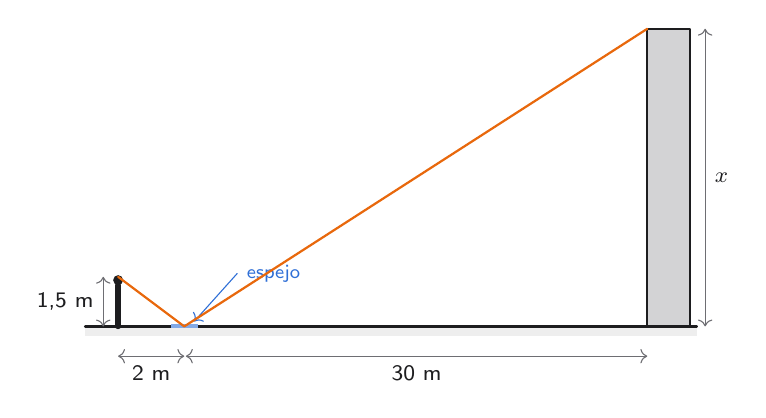
\begin{tikzpicture}[font=\small,x=0.42cm,y=0.42cm,line cap=round,line join=round,step={(1,1)}]
\fill[gris!12] (-1,-0.3) rectangle (17.5,0); \draw[tinta,thick] (-1,0)--(17.5,0);
\draw[tinta,line width=2pt] (0,0)--(0,1.25); \fill[tinta] (0,1.4) circle (0.15);
\filldraw[fill=gris!30,draw=tinta,thick] (16,0) rectangle (17.3,9);
\fill[azul!60] (1.6,-0.06) rectangle (2.4,0.06); \draw[azul,<-] (2.3,0.15)--(3.6,1.6) node[right,font=\scriptsize] {espejo};
\draw[nar,thick] (0,1.5)--(2,0)--(16,9);
\draw[<->,gris] (-0.45,0)--(-0.45,1.5) node[midway,left,font=\footnotesize,text=tinta] {1,5 m};
\draw[<->,gris] (0,-0.9)--(2,-0.9) node[midway,below,font=\footnotesize,text=tinta] {2 m};
\draw[<->,gris] (2.05,-0.9)--(16,-0.9) node[midway,below,font=\footnotesize,text=tinta] {30 m};
\draw[<->,gris] (17.75,0)--(17.75,9) node[midway,right,font=\footnotesize,text=tinta] {$x$};
\end{tikzpicture}
\end{document}
